\documentclass[tikz, margin=3.5mm]{standalone}
\usepackage{pgfplots}
\pgfplotsset{compat=newest}

\begin{document}
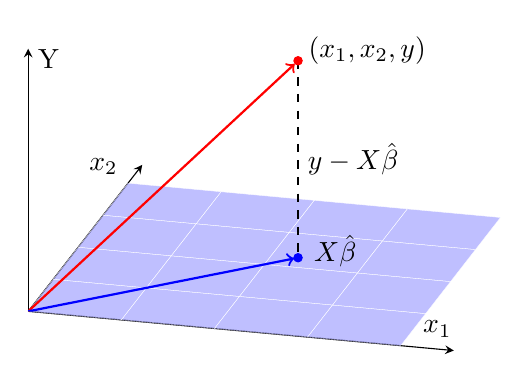
\begin{tikzpicture}
\begin{axis}[
    view={15}{30},
    axis lines=center,
    xlabel={\(x_1\)},
    ylabel={\(x_2\)},
    zlabel={Y},
    xmin=0, xmax=4,
    ymin=0, ymax=4,
    zmin=0, zmax=4,
    xtick=\empty,
    ytick=\empty,
    ztick=\empty,
]

% Drawing the plane
\fill[blue!50,opacity=0.5] (0,0,0) -- (3.5,0,0) -- (3.5,3.5,0) -- (0,3.5,0) -- cycle;
\addplot3[mesh, white!20, line width = .1pt, domain=0:3.5, samples=5, domain y=0:3.5, samples y=5, forget plot] {0};

% Drawing the projection line
\addplot3 [->, red, thick, shorten >=.6mm] coordinates {(0, 0, 0) (2, 2, 3)};
\addplot3 [->, blue, thick, shorten >=.5mm] coordinates {(0, 0, 0) (2, 2, 0)};
\draw [dashed] (2, 2, 3) -- node[midway, right] {\( y - X \hat \beta \)} (2, 2, 0);
\addplot3 [mark=*, red, mark size = 1.5pt] coordinates {(2, 2, 3)};
\addplot3 [mark=*, blue, mark size = 1.5pt] coordinates {(2, 2, 0)};
\node at (2.35,2,0.15) {$X \hat \beta$};
\node at (2.65,2,3.25) {$(x_1, x_2, y)$};

\end{axis}
\end{tikzpicture}
\end{document}
